\section{Organization}

\subsection{Mindmap}
In order to get a first impression of the problem a mindmap is used (see
figure \vref{fig:mindmap}).

\begin{figure}[htb]
\centering
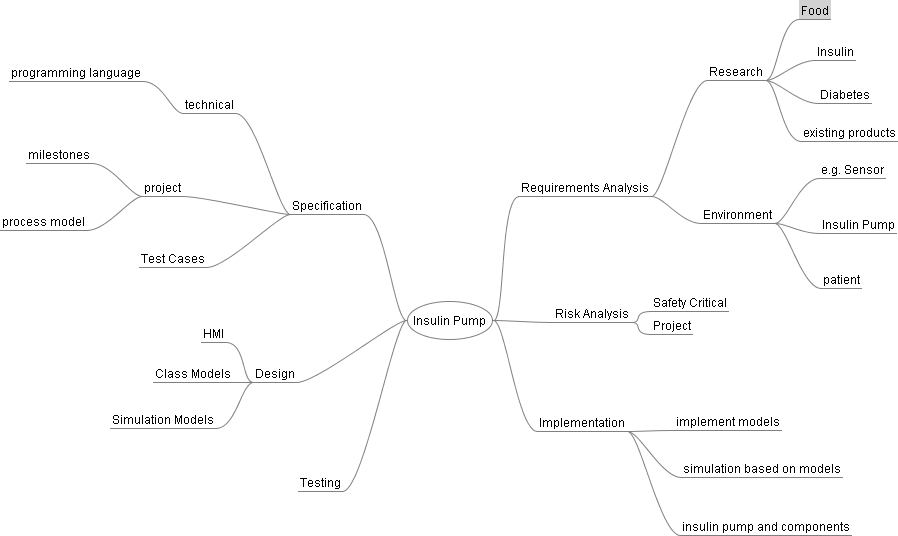
\includegraphics[width=\textwidth]{images/Insulin_Pump_Mindmap.png}
\caption{Mindmap of the problem}
\label{fig:mindmap}
\end{figure}

\newpage
\subsection{Development Process Model}
The spiral model is used for the main parts of our development.
See the project plan (see figures \vref{fig:projectplan1} and \vref{fig:projectplan2}) and the
mind map (see figure \vref{fig:mindmap}) for more detail.

\begin{figure}[htb]
\centering
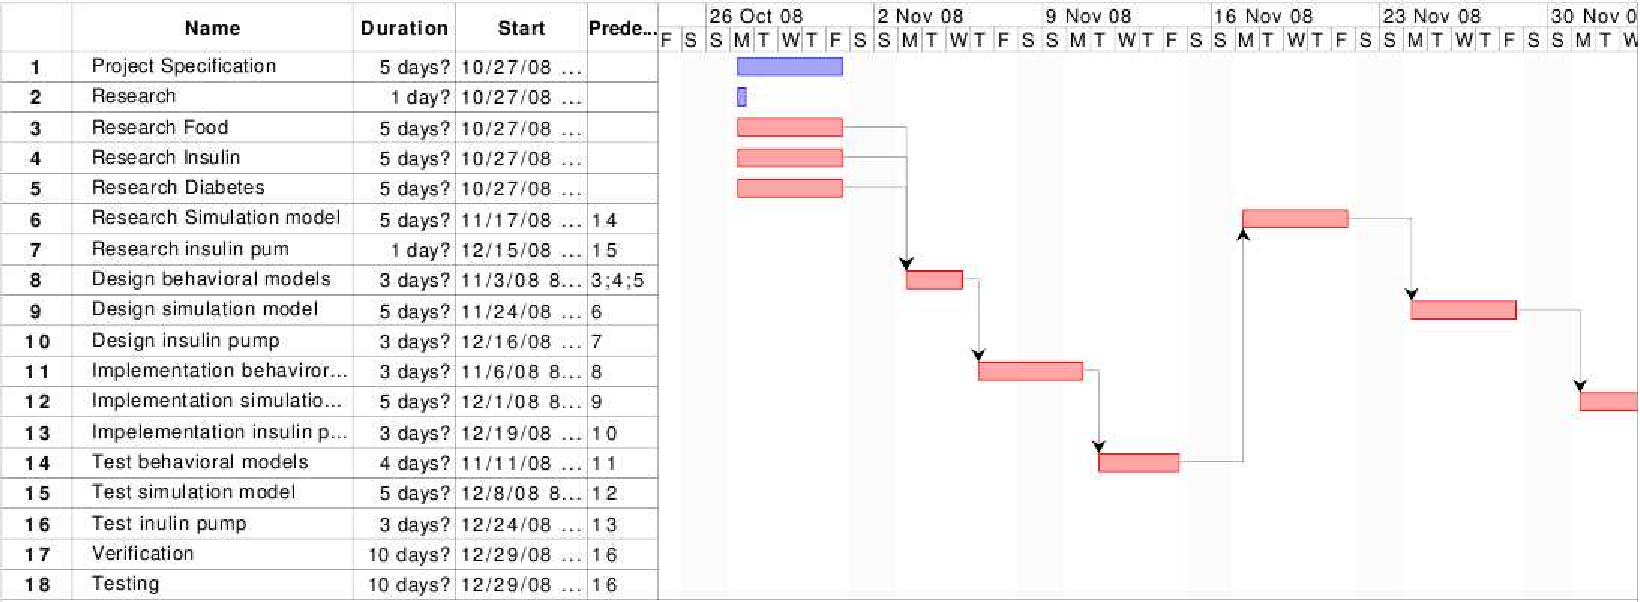
\includegraphics[width=\textwidth]{images/projectplan_page1}
\caption{Project Plan Page 1}
\label{fig:projectplan1}
\end{figure}

\begin{figure}[htb]
\centering
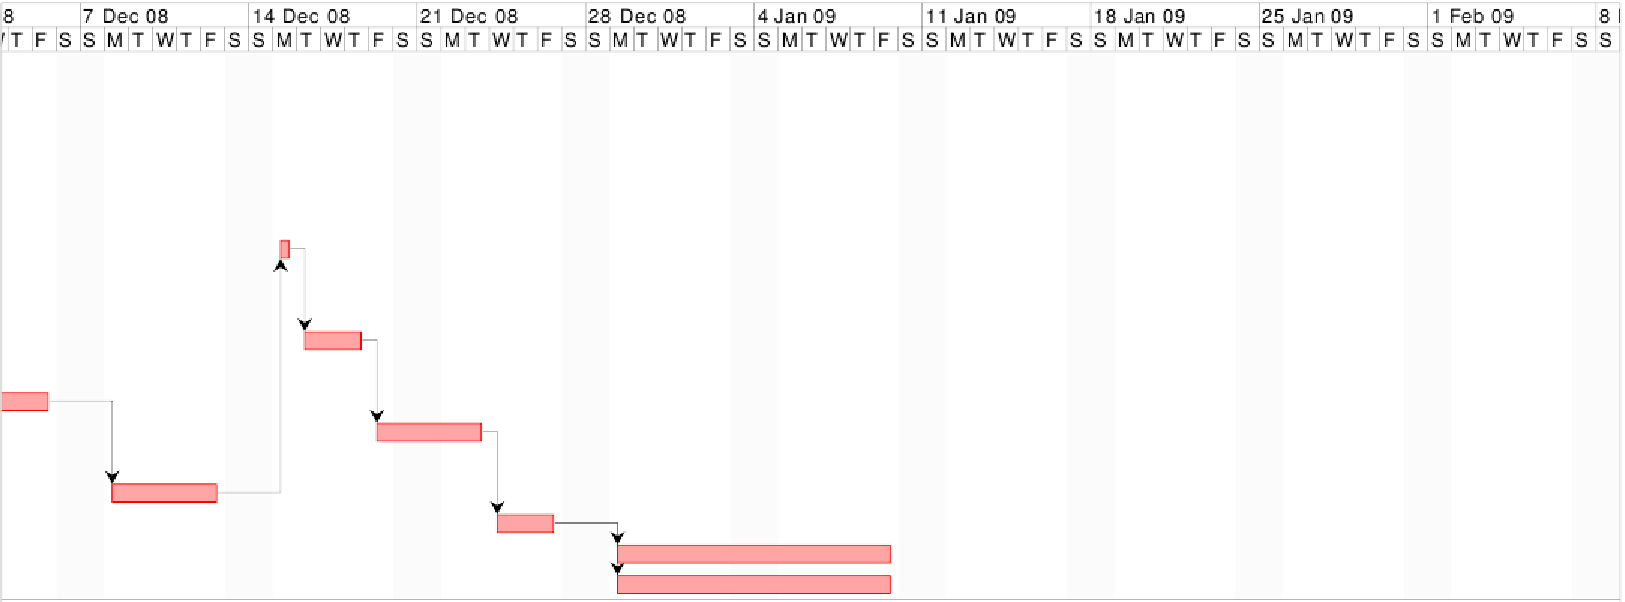
\includegraphics[width=\textwidth]{images/projectplan_page2}
\caption{Project Plan Page 2}
\label{fig:projectplan2}
\end{figure}

\newpage
At the end of November / the beginning of December quite a lot of work has
already been put into the Insulin Pump project.
Though it was not possible to follow the proposed project plan.
The following two figures show the now actual project plan (see figure
\vref{fig:projectplan_v3_1} and \vref{fig:projectplan_v3_2}):

\begin{figure}[htb]
\centering
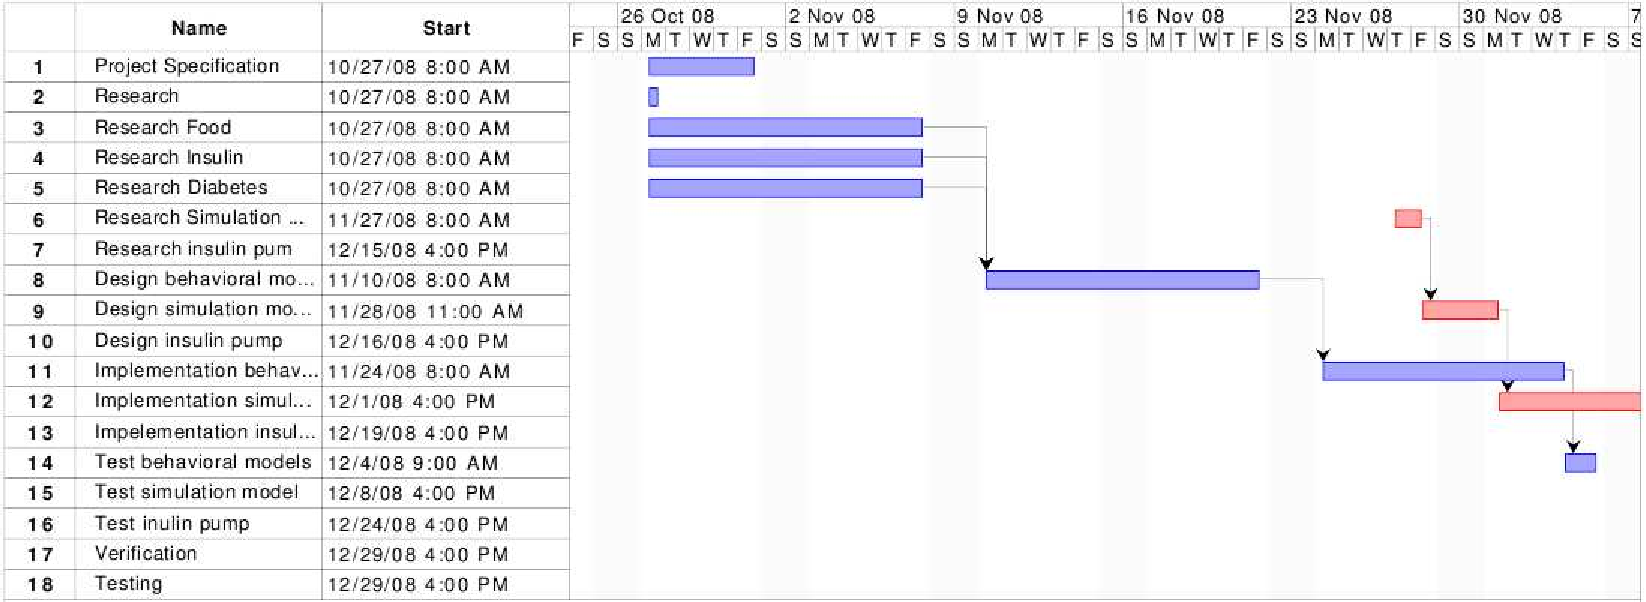
\includegraphics[width=\textwidth]{images/projectplan_v3_page1}
\caption{Project Plan (November/Dezember) Page 1}
\label{fig:projectplan_v3_1}
\end{figure}

\begin{figure}[htb]
\centering
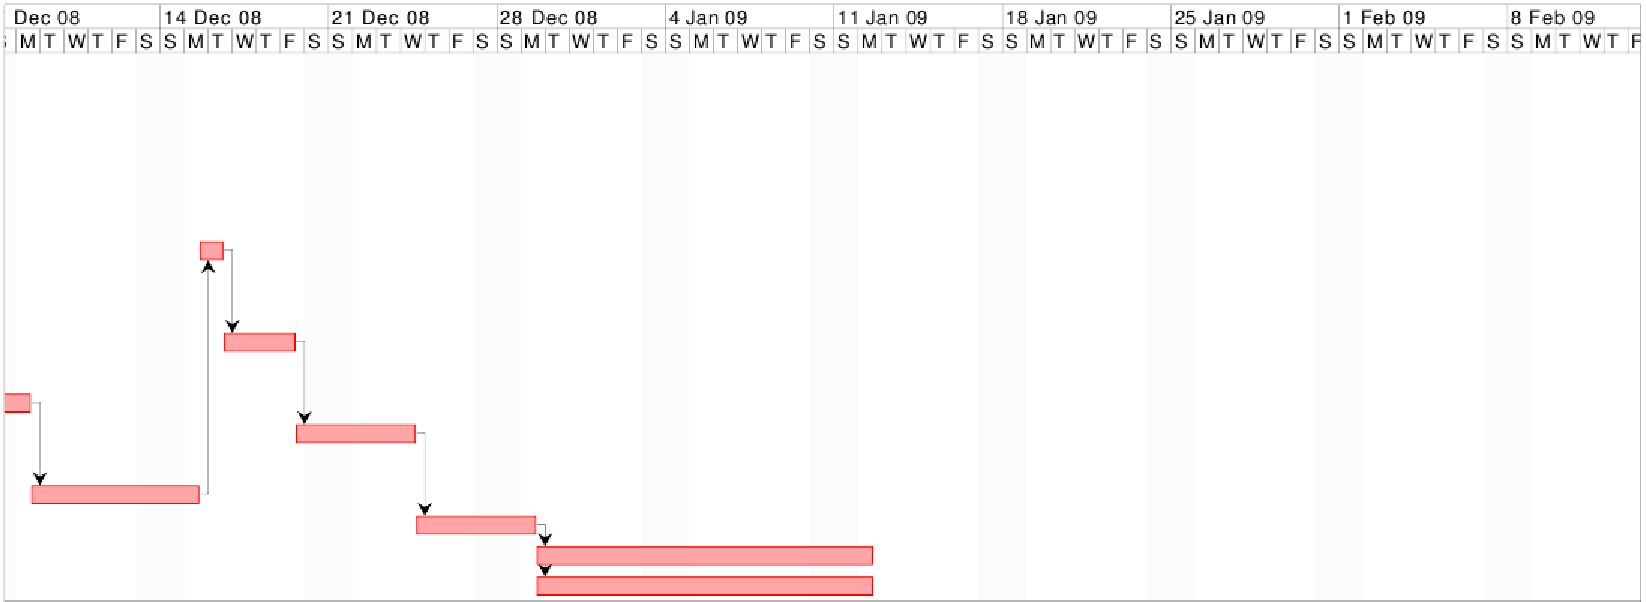
\includegraphics[width=\textwidth]{images/projectplan_v3_page2}
\caption{Project Plan (November/Dezember) Page 2}
\label{fig:projectplan_v3_2}
\end{figure}

This project plan shows now no connection from the testing of the behavioral
models to the research of the simulation.
This is because in this stage some tasks are now engaged in parallel and it was
not possible to display this other then this in the project plan.
This parallel process was mainly caused by different status in the groups
implementing the different behavioral models.

Also in order to catch up with the scheduled project plan further
simplifactions are introduced.
This has the purpose to deliver a working (but further simplified) product in
the end of the semester.

\subsection{Standardization}
Common value for measuring the blood glucose level is "mmol/l".
Programming language is Java.

\subsection{Specifications}
What do we want to achieve?
Simulation of the human body with diabetes and simulation of insulin pump.
Insulin pump has a sensor and automatic as well as manual injection.

\subsection{Risks}
People might get harmed or killed.
Project doesn't complete.

\subsubsection{Risk Handling}
Low glucose levels result in more serious effects on the health or even life then high levels.
So high glucose levels are prefered if there are situations when no clear preference can be made or one is in doubt.